\chapter{Baza podataka}


  
\section{ER model}

Za konceptualno modeliranje baze podataka najprije je definiran entitetsko-relacijski model koji pomoću entiteta predstavlja objekte u stvarnom svijetu. Svaki entitet opisan je svojim atributima. Posebno se definira ključni atribut koji definira svojstvo koje identificira entitet. Relacije opisuju kako su entiteti međusobno povezani. Na slici 2.1. možemo vidjeti grafički prikaz ER modela. Svaki entitet prikazan je pravokutnikom, a njegovi atributi elipsama. Relacije su prikazane rombovima, a same veze linijama. Baza podataka ima sljedeće entitete


\begin{packed_item}
			\item Uloga
                \item Korisnik
                \item Slika
			\item Bilješka
			\item Teren
			\item SatiVožnje
			\item Dogadjaj
		\end{packed_item}

\noindent Svaki od prethodno  navedenih entiteta zadovoljava prvu, drugu i treću normalnu formu. Prva normalna forma zahtjeva da svi atributi sadrže nedjeljive vrijednosti i da svaki atribut ima jedinstveni identifikator. Druga normalna forma zahtjeva da svi neključni atributi zavise od cijelog primarnog ključa, ne samo jednog njegovog dijela. Na kraju, treća normalna forma zahtjeva nepostojanje tranzitivne zavisnosti, tj. zahtijeva da neključni atributi ne zavise od drugih neključnih atributa.



\begin{figure}[H]
					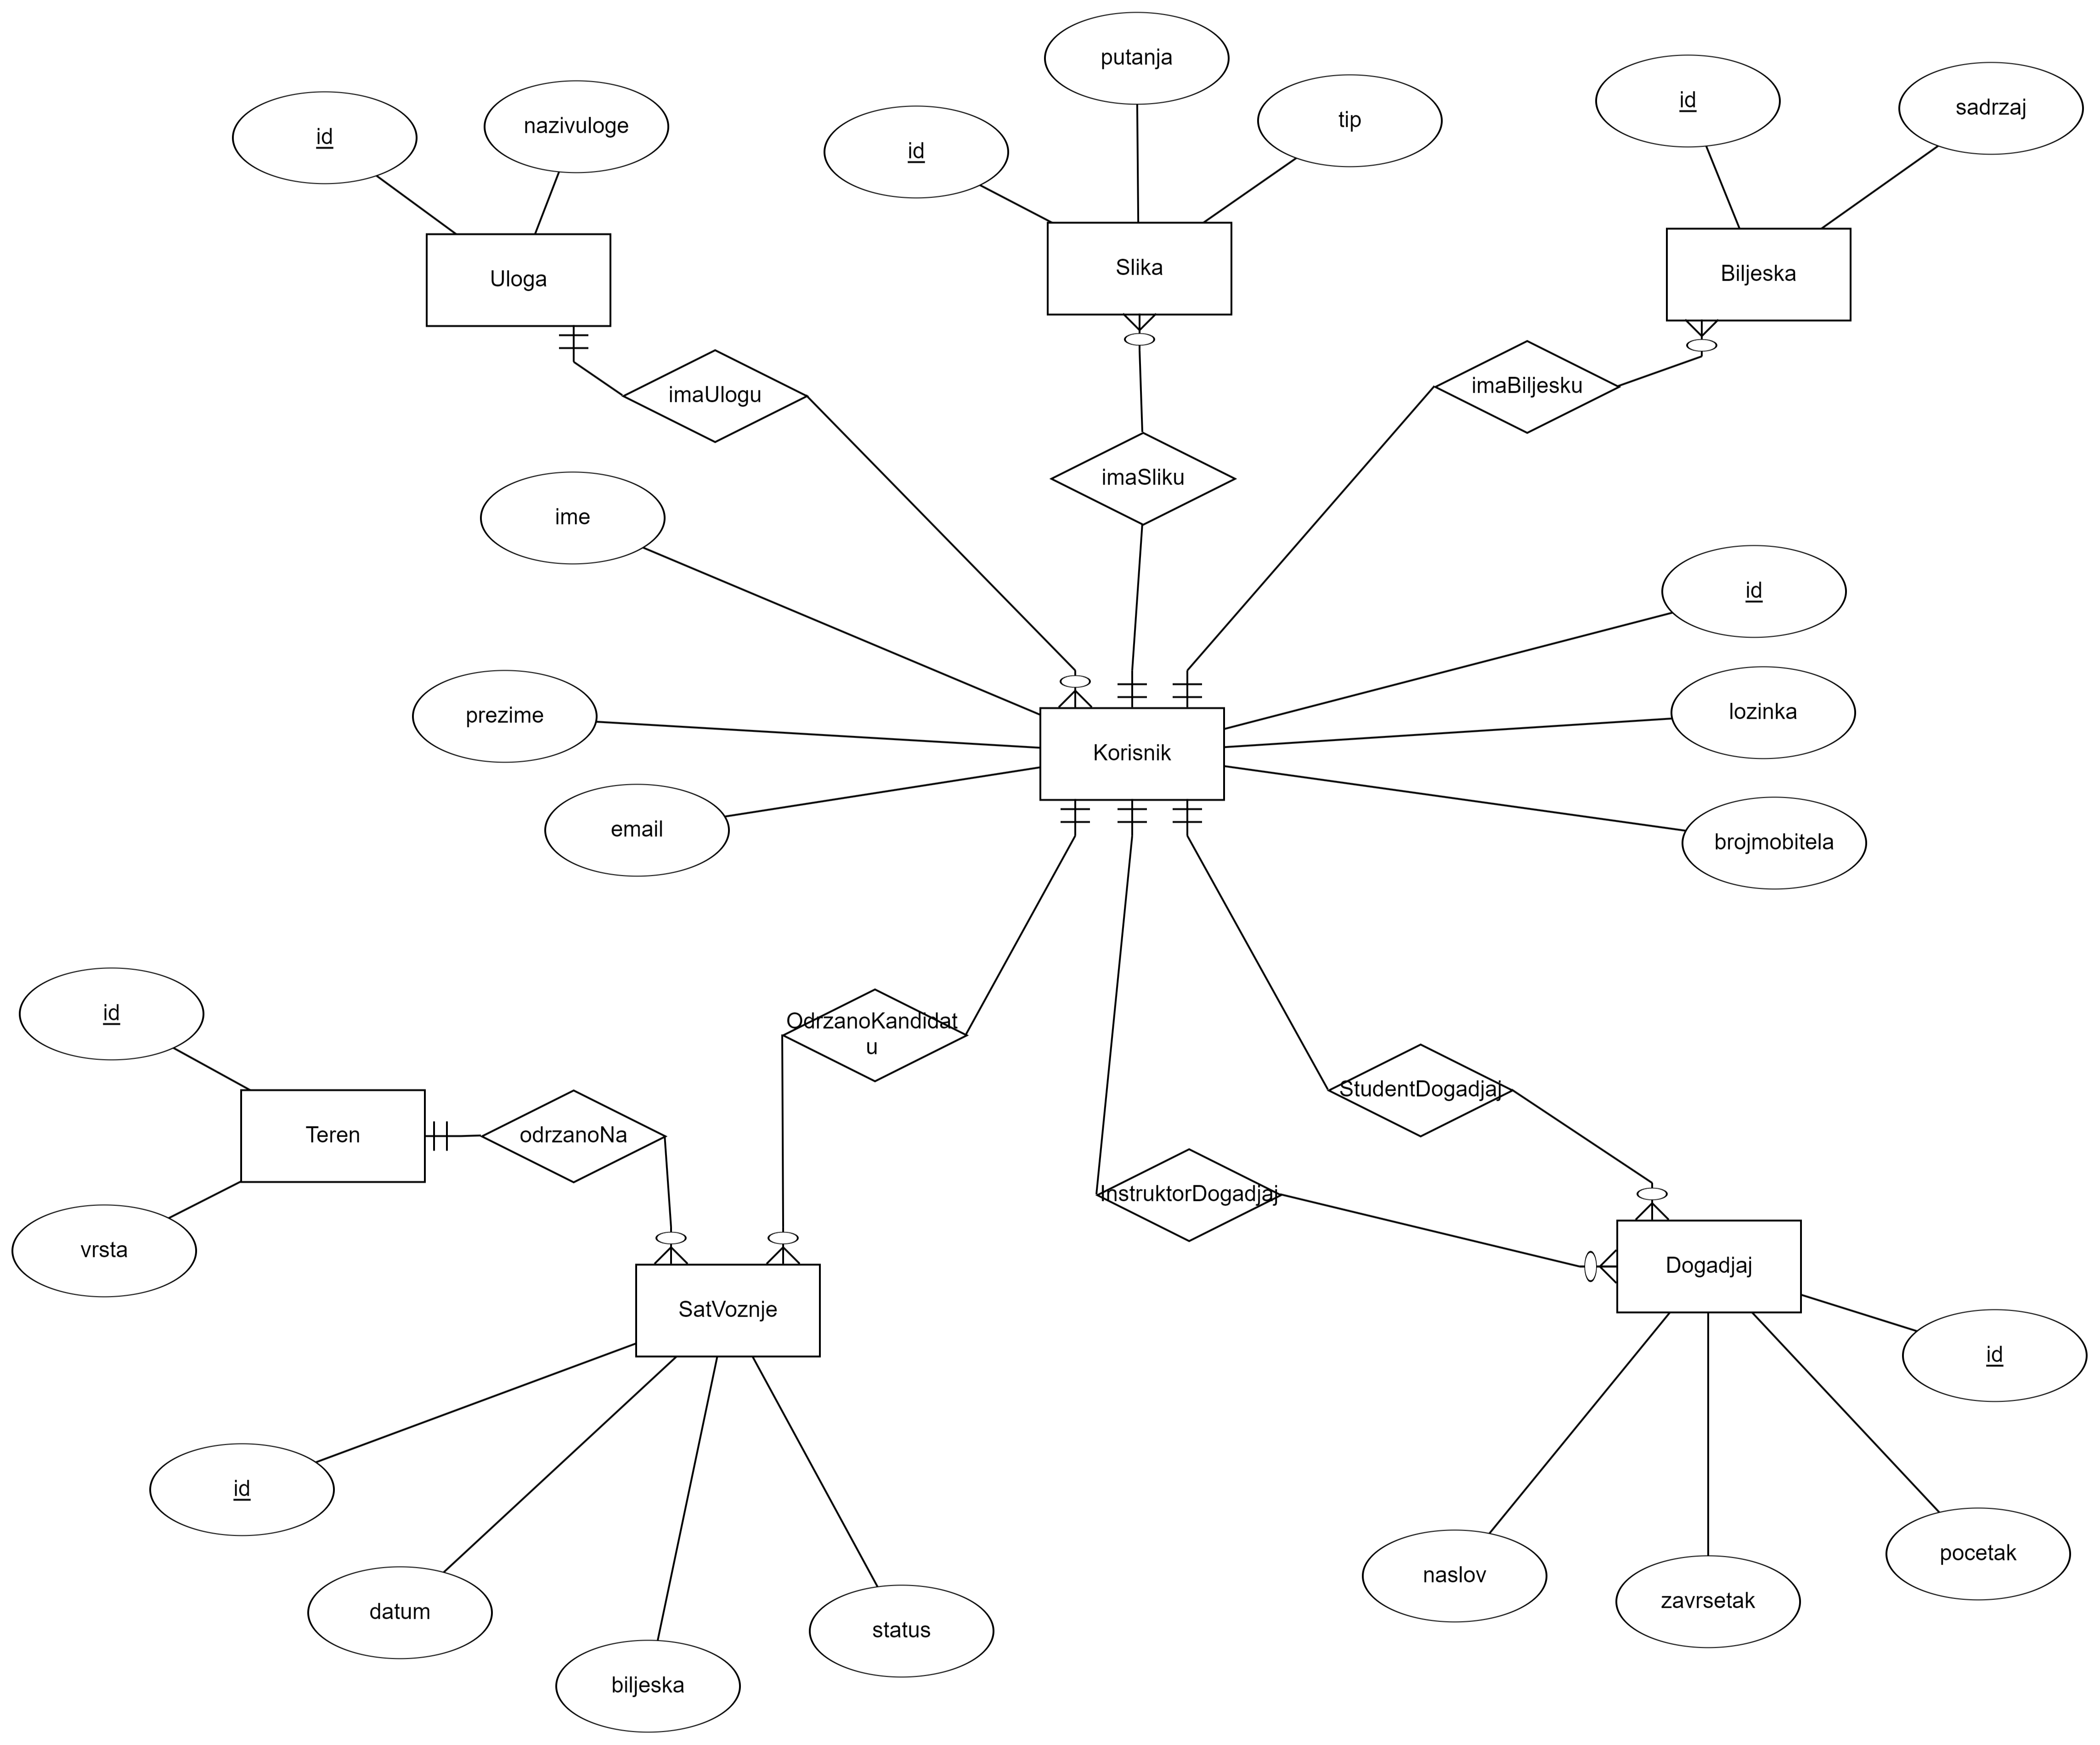
\includegraphics[width=\textwidth]{slike/ERBaza.png} 
					\centering
					\caption{ER dijagram baze podataka}
					\label{fig:promjene}
				\end{figure}




\noindent Svaki korisnik ima jedinstvenu ulogu, sliku i bilješku koja se odnosi samo na njega. Unos bilješke i slike za pojedinog korisnika nije obavezan, ali svaki registriran korisnik mora imati dodijeljenu ulogu. Sat vožnje može se održati na jednoj vrsti terena, dok se teren može povezati s više satova. Svakom korisniku može se održati više sati vožnje, ali jedan zapis vožnje odnosi se samo na jednog korisnika, odnosno kandidata. Događaj je povezan s korisnikom tako da se odnosi na minimalno jednog, a maksimalno dva korisnika. Postoje događaji koji se odnose samo na instruktora ili samo na kandidata, primjerice raspoloživost kandidata za održavanje obuke, dok sam termin održavanja obuke se odnosi i na kandidata i na instruktora. 


\section{Opis relacija}




 
 \noindent Entitet \textbf{Uloga}  sadrži informaciju o ulozi korisnika u sustavu. Svi atributi moraju biti definirani i unose se za svakog korisnika.

\label{tab:uloga}
\begin{longtblr}[
    label=none,
    entry=none
]{
    width = \textwidth,
    colspec = {|X[8,l]|X[6,l]|X[20,l]|},
    rowhead = 1
}
\hline 
\SetCell[c=3]{c}{\textbf{Uloga}} \\ \hline[3pt]
\SetCell{LightGreen}
ulogaID & BIGINT & jedinstveni identifikator uloge \\ \hline
nazivuloge & VARCHAR & opis korisničke uloge \\ \hline
\end{longtblr}



\noindent Entitet \textbf{Korisnik} sadrži korisničke podatke o svakom korisniku u sustavu. Svi atributi moraju biti definirani budući da entitet sadrži sve relevantne informacije o registriranom korisniku aplikacije.



\label{tab:korisnik}
\begin{longtblr}[
    label=none,
    entry=none
]{
    width = \textwidth,
    colspec = {|X[8,l]|X[6,l]|X[20,l]|},
    rowhead = 1
}
\hline 
\SetCell[c=3]{c}{\textbf{Korisnik}} \\ \hline[3pt]
\SetCell{LightGreen}
korisnikID & BIGINT & jedinstveni identifikator korisnika \\ \hline
ime & VARCHAR & ime korisnika \\ \hline
prezime & VARCHAR & prezime korisnika\\ \hline
email & VARCHAR & adresa elektroničke pošte \\ \hline
lozinka & VARCHAR & lozinka korisničkog računa \\ \hline
brojmobitela & VARCHAR & broj mobitela korisnika \\ \hline
\SetCell{LightBlue}ulogaID & BIGINT & jedinstveni identifikator uloge korisnika \\ \hline
\end{longtblr}



\noindent Entitet \textbf{Biljeska}  sadrži informaciju o bilješci za određenog korisnika u sustavu. Svi atributi moraju biti definirani i: obavezan unos za svakog korisnika.



\label{tab:biljeska}
\begin{longtblr}[
    label=none,
    entry=none
]{
    width = \textwidth,
    colspec = {|X[8,l]|X[6,l]|X[20,l]|},
    rowhead = 1
}
\hline 
\SetCell[c=3]{c}{\textbf{Bilješka}} \\ \hline[3pt]
\SetCell{LightGreen}
biljeskaID & BIGINT & jedinstveni identifikator bilješke \\ \hline
sadrzaj & VARCHAR & tekstualni zapis bilješke \\ \hline
\SetCell{LightBlue}korisnikID & BIGINT & jedinstveni identifikator korisnika \\ \hline
\end{longtblr}



\noindent Entitet \textbf{Slika}  sadrži putanju do slike određenog korisnika u sustavu. Svi atributi moraju biti definirani: obavezan unos za svakog korisnika.


\label{tab:slika}
\begin{longtblr}[
    label=none,
    entry=none
]{
    width = \textwidth,
    colspec = {|X[8,l]|X[6,l]|X[20,l]|},
    rowhead = 1
}
\hline 
\SetCell[c=3]{c}{\textbf{Slika}} \\ \hline[3pt]
\SetCell{LightGreen}
slikaID & BIGINT & jedinstveni identifikator zapisa \\ \hline
tip & VARCHAR & tip medijskog sadržaja (image) \\ \hline
putanja & VARCHAR & putanja do slike \\ \hline
\SetCell{LightBlue}korisnikID & BIGINT & jedinstveni identifikator korisnika  \\ \hline
\end{longtblr}




\noindent Entitet \textbf{Teren} sadrži informaciju o vrsti terena na kojoj je održan sat vožnje. Moguće vrijednosti su "V" - vježbalište koje označava održavanje sata na poligonu  i "C" - cesta koja označava održavanje sata na otvorenoj cesti. Svi atributi moraju biti definirani.


\label{tab:teren}
\begin{longtblr}[
    label=none,
    entry=none
]{
    width = \textwidth,
    colspec = {|X[8,l]|X[6,l]|X[20,l]|},
    rowhead = 1
}
\hline 
\SetCell[c=3]{c}{\textbf{Teren}} \\ \hline[3pt]
\SetCell{LightGreen}
terenID & BIGINT & jedinstveni identifikator terena \\ \hline
vrsta & VARCHAR & vrsta terena \\ \hline
\end{longtblr}





\noindent Entitet \textbf{SatVoznje} sadrži informaciju o održanom satu vožnje uključujući polaznika autoškole i teren na kojem je održan sat vožnje. Navedeni atributi predstavljaju zapravo strane ključeve. Svi atributi moraju biti definirani.

\label{tab:satvoznje}
\begin{longtblr}[
    label=none,
    entry=none
]{
    width = \textwidth,
    colspec = {|X[8,l]|X[6,l]|X[20,l]|},
    rowhead = 1
}
\hline 
\SetCell[c=3]{c}{\textbf{SatVoznje}} \\ \hline[3pt]
\SetCell{LightGreen}
satID & BIGINT & jedinstveni identifikator održanog sata \\ \hline
datum & DATE & datum održanog sata\\ \hline
biljeska & VARCHAR & komentar od strane instruktora \\ \hline
status & VARCHAR & status \\ \hline
\SetCell{LightBlue}kandidatID & BIGINT & jedinstveni identifikator kandidata kojem je održan sat obuke \\ \hline
\SetCell{LightBlue}terenID & BIGINT & jedinstveni identifikator terena na kojem je održan sat \\ \hline
\end{longtblr}



\noindent Entitet \textbf{Dogadjaj}  sadrži informaciju o pojedinom zapisu u kalendaru kandidata i instruktora. Jedinstveni identifikatori kandidata i instruktora su strani ključevi. Budući da svaki korisnik može sam unositi događaje u svoj kalendar, te instruktor može kandidatu zakazati sat, određeni zapisi mogu imati oba strana ključa definirana, dok je dozvoljeno izostavljanje jednog od ključeva ovisno u korisniku koji unosi događaj

\begin{longtblr}[
    label=none,
    entry=none
]{
    width = \textwidth,
    colspec = {|X[8,l]|X[6,l]|X[20,l]|},
    rowhead = 1
}
\hline 
\SetCell[c=3]{c}{\textbf{Dogadjaj}} \\ \hline[3pt]
\SetCell{LightGreen}
dogadjajID & BIGINT & jedinstveni identifikator događaja \\ \hline
pocetak & TIMESTAMP & datum održanog sata\\ \hline
zavrsetak & TIMESTAMP & naziv terena \\ \hline
naslov & VARCHAR & naslov događanja\\ \hline
\SetCell{LightBlue}kandidatID & BIGINT & jedinstveni identifikator kandidata  \\ \hline
\SetCell{LightBlue}instruktorID & BIGINT & jedinstveni identifikator instruktora \\ \hline


\end{longtblr}


\section{Relacijski model}


     
Na slici 3.1. možemo vidjeti relacijsku shemu baze podataka. 
\begin{figure}[H]
					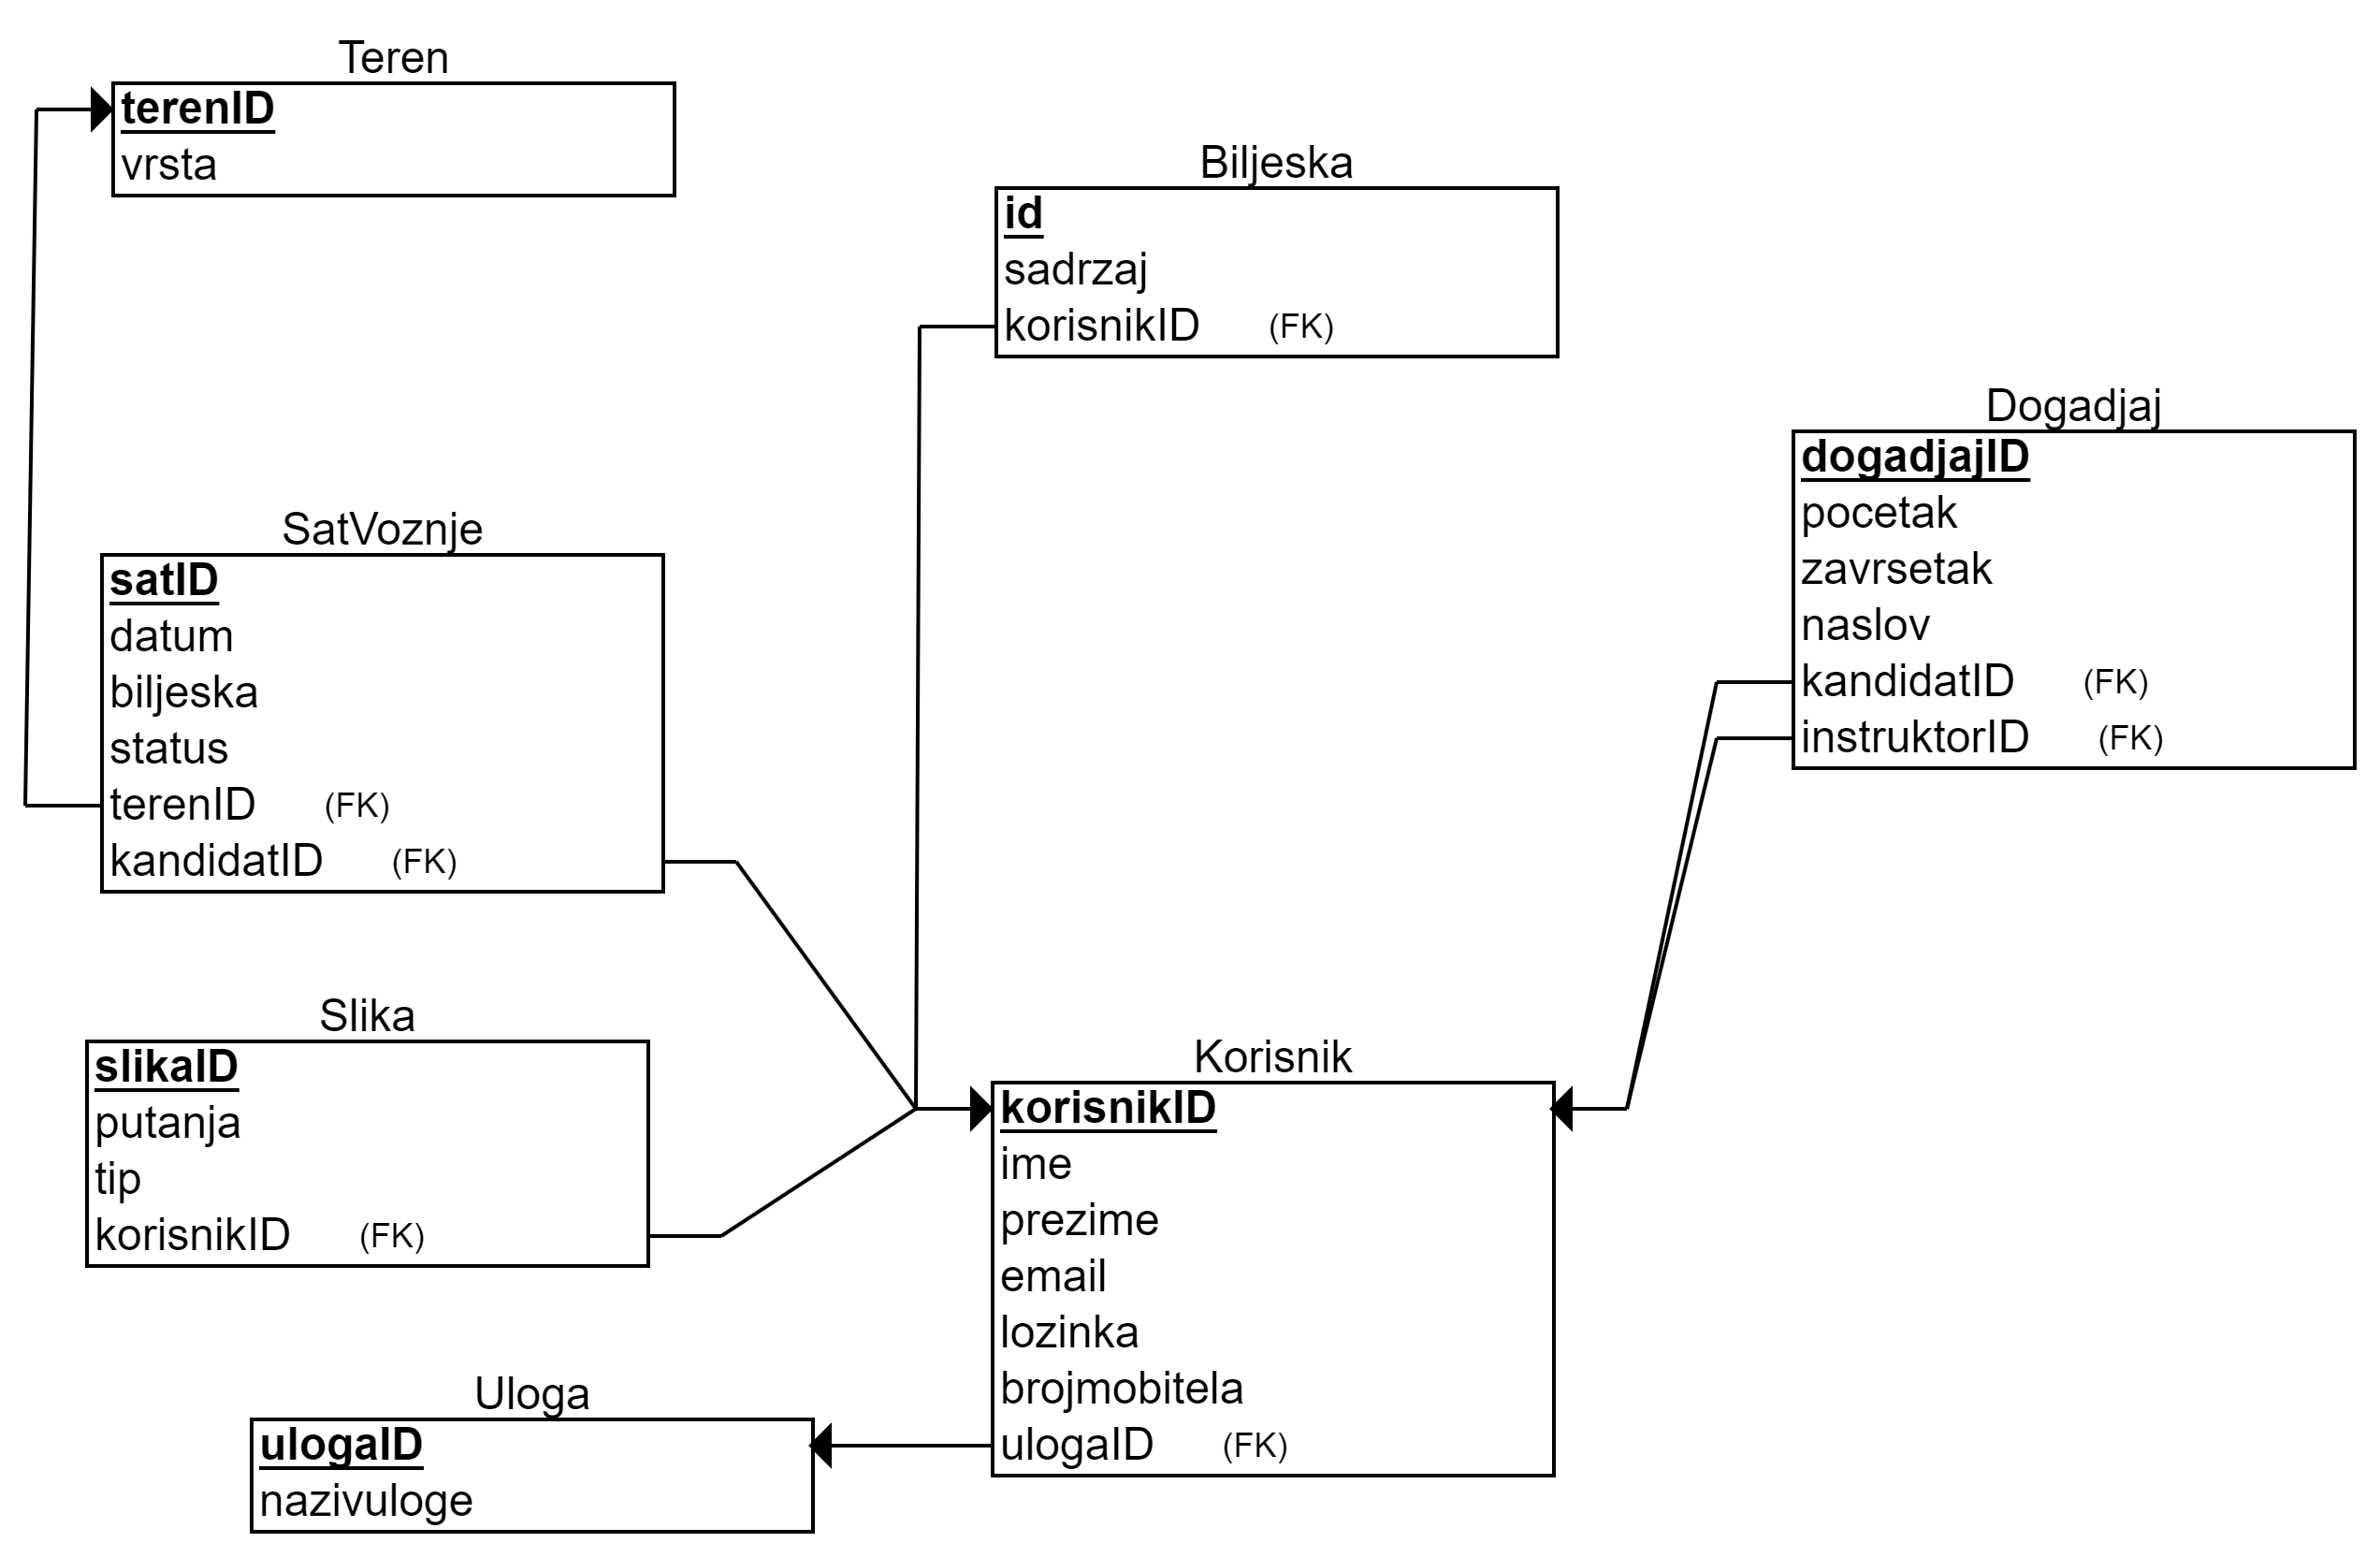
\includegraphics[width=\textwidth]{slike/RelBaza.png} 
					\centering
					\caption{Dijagram baze podataka}
					\label{fig:promjene}
				\end{figure}


\noindent Sustav koristi H2 relacijsku bazu podataka koja se posebno ističe po lakoj integraciji s aplikacijama razvijenim u programskom jeziku Java. Glavna karakteristika aplikacije je njena brzina i učinkovitost zbog organizacije i pohrane podataka u radnu memoriju, dok se inače u sustavima za upravljanje podacima koriste mehanizmi za pohranu na disku. Kao takva, H2 baza pruža podršku standardnim SQL naredbama. Razvoj i testiranje same baze posebno olakšava i grafičko korisničko sučelje kojem se pristupa putem weba. Iako je H2 odličan izbor za razvojne faze projekta, koristit će se i u proizvodnom okruženju web aplikacije zbog manjih zahtjeva na bazu podataka. Budući da u sustavu postoje samo tri uloge korisnika, zbog jednostavnosti u implementaciji su združeni entiteti \noindent \textbf{Korisnik} i \noindent \textbf{Uloga}. Iz istog razloga združeni su i entiteti \noindent \textbf{Teren} i \noindent \textbf{SatVoznje}. U konačnici, implementacija aplikacije je realizirana pomoću pet entiteta: \noindent \textbf{Korisnik}, \noindent 
    \textbf{Slika},  \noindent
     \textbf{Bilješka}, \noindent \textbf{SatVožnje}, \noindent \textbf{Dogadjaj}.




